\subsection{How to Sketch Polynomial Functions}
Here's how to sketch a graph of a polynomial function with $x$-intercepts, $y$-intercept, multiplicity, and end behaviour.

\textbf{Note: }Maximum turning points are always $\text{Degree } - 1 $.

\begin{example}[Polynomial Function Sketch]
  \hfill
  \begin{enumerate}
  \item $h(x) = -2(x - 7)\left(x + \frac{1}{2}\right)^2(x + 4)^3(x^2 + 9)^2$ \\
    $-2 \cdot x^1 \cdot x^2 \cdot x^3 \cdot x^4$
    \begin{enumerate}
    \item Leading term: $-2x^{10}$
      \begin{enumerate}
      \item Degree: $10$
      \item Max turning point: $9$
      \item End behaviour: Downward even graph.
      \end{enumerate}
    \item $y$-intercept: $(0, 18144)$
    \item $x$-intercept: $-2(x - 7)\left(x + \frac{1}{2}\right)^2(x + 4)^3(x^2 + 9)^2 = 0$ \\
      $x - 7 = 0 \quad x + \frac{1}{2} = 0 \quad  x + 4 = 0 \quad x^3 + 9 = 0$ \\
      $x = 7 \text{ mult 1 }\quad x = -\frac{1}{2} \text{ mult 2 } \quad x = -4 \text{ mult 3 }\quad x^2 + 9 = 0 \to \text{ No x-intercept }$ \\
      $x = 7 \to$ Cross the $x$ axis. \\
      $x = -\frac{1}{2} \to$ Bounce/touch the $x$ axis. \\
      $x = -4 \to $ Cross the $x$ axis. \\
    \end{enumerate}
  \item $f(x) = x^2(x - 3)$ \\
    $x^2 \cdot x$ \\
    \begin{enumerate}
    \item Leading term: $x^3$
      \begin{enumerate}
      \item Degree: $3$
      \item Max turning point: $2$
      \item End behaviour: Odd graph.
      \end{enumerate}
    \item $y$-intercept: $(0, 0)$ 
    \item $x$-intercept: $x = 0 \text{ mult 2 }\quad x - 3 = 0 \to x = 3 \text{ mult 1 }$ \\
    \item Graph:
      \begin{center}
        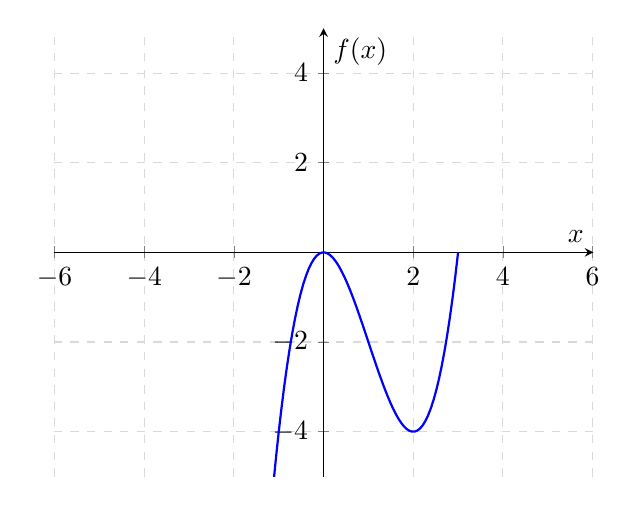
\begin{tikzpicture}
          \begin{axis}[
	      axis lines = center,
	      xlabel = $x$,
	      ylabel = $f(x)$,
	      xmin = -5, xmax = 5,
	      ymin = -5, ymax = 5,
              restrict y to domain = -20:10,
	      grid = major,
	      grid style = {dashed, gray!30},
	      axis equal
	    ]
	    \addplot [domain=-3:3, samples=100, thick, blue] {x^2*(x-3)};
          \end{axis}
        \end{tikzpicture}
      \end{center}
    \end{enumerate}
  \item $f(x) = -2(x + 2)(x - 2)^3$
    $-2 \cdot x^1 \cdot x^3$
    \begin{enumerate}
    \item Leading term: $-2x^4$
      \begin{enumerate}
      \item Degree: $4$
      \item Max turning point: $3$
      \item End behaviour: Downward even graph.
      \end{enumerate}
    \item $y$-intercept: $(0, 32)$
    \item $x$-intercept: $-2(x + 2)(x - 2)^3 = 0$ \\
      $x + 2 = 0 \quad x -2 = 0$ \\
      $x = -2 \text{ mult 1 }\quad x = 2 \text{ mult 3 }$ \\
      $x = -2$ crosses the $x$ axis. \\
      $x = 2$ crosses the $x$ axis.
    \item Graph:
      \begin{center}
        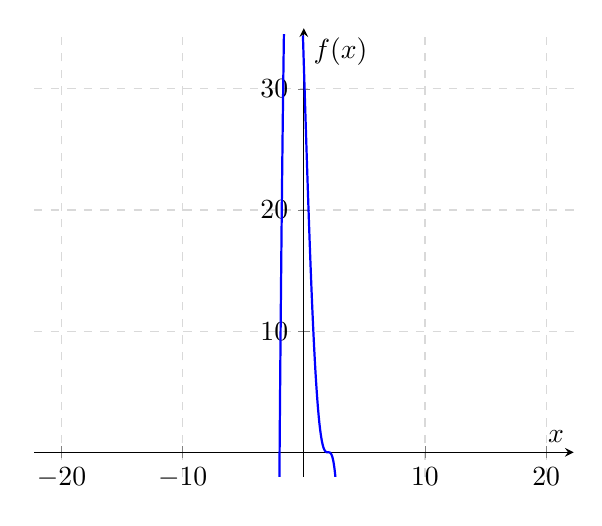
\begin{tikzpicture}
          \begin{axis}[
	      axis lines = center,
	      xlabel = $x$,
	      ylabel = $f(x)$,
	      xmin = -20, xmax = 20,
	      ymin = -2, ymax = 35,
              restrict y to domain = -10:35,
	      grid = major,
	      grid style = {dashed, gray!30},
	      axis equal
	    ]
	    \addplot [domain=-3:3, samples=200, thick, blue] {-2*(x+2)*(x-2)^3};
          \end{axis}
        \end{tikzpicture}
      \end{center}
    \end{enumerate}
  \item $h(x) = (x + 4)^2(1 - x)$
    \textbf{Note: }We factor the sign here to avoid sign errors.
    $(-x + 1)$ \\
    $-(x - 1)$ \\
    $h(x) = -(x + 4)^2(x - 1)$ \\
    $-1 \cdot x^2 \cdot x$
    \begin{enumerate}
    \item Leading term: $-1x^3$
      \begin{enumerate}
      \item Degree: $3$
      \item Max turning point: $2$
      \item End behaviour: Reflected odd graph.
      \end{enumerate}
    \item $y$-intercept: $(0, 16)$
    \item $x$-intercept: $x + 4 = 0 \quad x - 1 =0$ \\
      $x = -4 \text{ mult 1 }\quad x = 1 \text{ mult 1 }$\\
      $x = -4$ bounces upon the graph. \\
      $x = 1$ crosses the graph.
    \item Graph:
      \begin{center}
        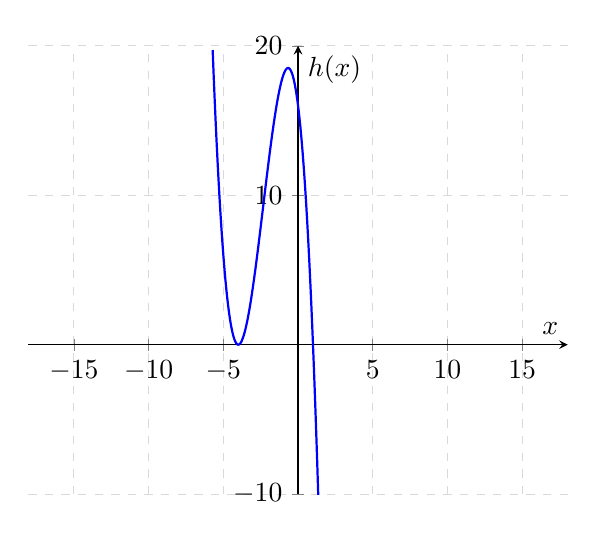
\begin{tikzpicture}
          \begin{axis}[
	      axis lines = center,
	      xlabel = $x$,
	      ylabel = $h(x)$,
	      xmin = -10, xmax = 10,
	      ymin = -10, ymax = 20,
              restrict y to domain = -20:20,
	      grid = major,
	      grid style = {dashed, gray!30},
	      axis equal
	    ]
	    \addplot [domain=-8:5, samples=200, thick, blue] {(x+4)^2*(1-x)};
          \end{axis}
        \end{tikzpicture}
      \end{center}
    \end{enumerate}
  \item $f(x) = -5x(x^2 - 4)(x + 3)$ \\
    $f(x) = -5x(x - 2)(x + 2)(x + 4)$ \\
    $-5 \cdot x \cdot x \cdot x \cdot x$ \\
    \begin{enumerate}
    \item Leading Term: $-5x^4$
      \begin{enumerate}
      \item Degree: $4$
      \item Max turning point: $3$
      \item End behaviour: Downward even graph.
      \end{enumerate}
    \item $y$-intercept: $(0, 0)$
    \item $x$-intecept: $x = 0 \quad x - 2 = 0 \quad x + 2 = 0 \quad x + 3 = 0$ \\
      \textbf{Note: }Everything here has a multiplicity of 1. \\
      $x = 0 \quad x = 2 \quad x = -2 \quad x = -3$ \\
      $x = 0$ crosses the gap. \\
      $x = 2$ crosses the gap. \\
      $x = -2$ crosses the gap. \\
      $x = -3$ crosses the gap.
    \item Graph:
      \begin{center}
        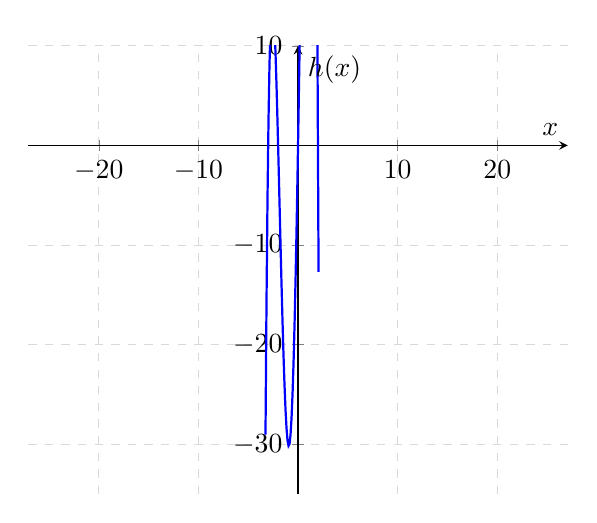
\begin{tikzpicture}
          \begin{axis}[
	      axis lines = center,
	      xlabel = $x$,
	      ylabel = $h(x)$,
	      xmin = -10, xmax = 10,
	      ymin = -35, ymax = 10,
              restrict y to domain = -32:30,
	      grid = major,
	      grid style = {dashed, gray!30},
	      axis equal
	    ]
	    \addplot [domain=-10:10, samples=200, thick, blue] {-5*x*(x^2-4)*(x+3)};
          \end{axis}
        \end{tikzpicture}
      \end{center}
    \end{enumerate}
  \item $g(x) = 2(x - 1)^2(x^2 - 16)$ \\
    $2(x - 1)^2(x - 4)(x + 4)$ \\
    $2 \cdot x^2 \cdot x \cdot x$
    \begin{enumerate}
    \item Leading Term: $2x^4$
      \begin{enumerate}
      \item Degree: $4$
      \item Max turning point: $3$
      \item End behaviour: $Even graph.$
      \end{enumerate}
    \item $y$-intercept: $(0,  -32)$
    \item $x$-intecept: $x - 1 = 0 \quad x - 4 = 0 \quad x + 4 = 0$ \\
      $x = 1 \text{ mult 2 }\quad x = 4 \text{ mult 1 } \quad x = -4 \text{ mult 1 }$ \\
      $x = 1$ bounces upon the graph. \\
      $x = 4$ crosses the graph. \\
      $x = -4$ crosses the graph.
    \item Graph:
      \begin{center}
        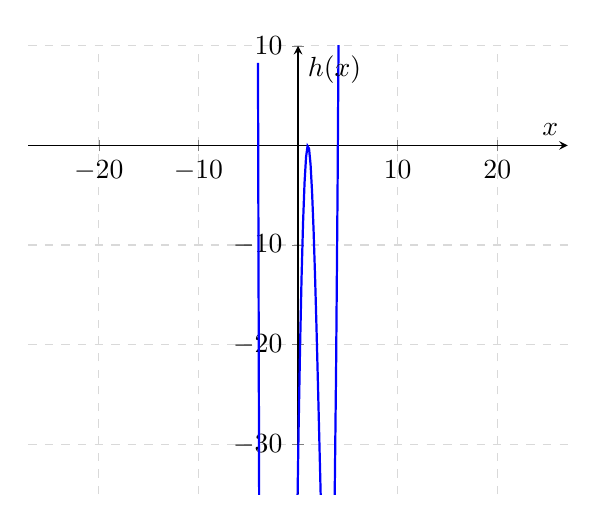
\begin{tikzpicture}
          \begin{axis}[
	      axis lines = center,
	      xlabel = $x$,
	      ylabel = $h(x)$,
	      xmin = -10, xmax = 10,
	      ymin = -35, ymax = 10,
              restrict y to domain = -70:20,
	      grid = major,
	      grid style = {dashed, gray!30},
	      axis equal
	    ]
	    \addplot [domain=-20:10, samples=200, thick, blue] {2*(x-1)^2*(x^2-16)};
          \end{axis}
        \end{tikzpicture}
      \end{center}
    \end{enumerate}
  \end{enumerate}
\end{example}
